\documentclass[14pt]{book}

\usepackage{fancyhdr}
\usepackage{graphicx}
\usepackage[margin=2.5cm]{geometry}
\usepackage{graphicx}
\usepackage{anysize}
\usepackage{xcolor}
\usepackage{caption}
\usepackage{subcaption}

\marginsize{2cm}{2cm}{2cm}{2cm} % Izquierda, derecha, arriba, abajo
\setlength{\parindent}{0cm}
\pagestyle{fancy}
\fancyhf{}
\fancyhead[L]{\footnotesize Compiladores} %encabezado izquierda
\fancyhead[R]{\footnotesize David Pérez Jacome}   % derecha
\fancyfoot[L]{\footnotesize}  %izquierda
\fancyfoot[C]{Página \thepage}
\renewcommand{\footrulewidth}{0.4pt}

\begin{document}
\begin{center}
  \newcommand{\HRule}{\rule{\linewidth}{0.5mm}}
  \begin{minipage}{0.48\textwidth}
    \begin{flushleft}
      
\includegraphics[scale = 0.08]{images/logo_unam.png}
    \end{flushleft}
  \end{minipage}
  \begin{minipage}{0.48\textwidth}
    \begin{flushright}
      
\includegraphics[scale =0.22]{images/logo_ciencias.png}
    \end{flushright}
  \end{minipage}
  \vspace*{-1.5cm}
  \textsc{\huge Nacional Autónoma de México \\ \vspace{-4px} Universidad }\\[2cm]
  \textsc{\LARGE Facultad de Ciencias}\\[1.5cm]
  \begin{minipage}{0.9\textwidth}
    \begin{center}
      \textsc{\LARGE Compiladores}
    \end{center}
  \end{minipage}\\[0.5cm]
  \vspace*{1cm}
  \HRule \\[0.4cm]
  { \huge \bfseries Examen casa}\\[0.4cm]
  \HRule \\[1.5cm]
  \begin{minipage}{0.52\textwidth}
    \begin{flushleft} \large \small \vspace{-0.6cm} \vspace{-0.6cm}
      Alumno David Pérez Jacome \\
    \end{flushleft}
  \end{minipage}
  \begin{minipage}{0.46\textwidth}
    \vspace{-0.6cm}
    \begin{flushright} \large \small \emph{Profesor:}
      Miguel Carrillo Barajas \\
    \end{flushright}
  \end{minipage}
  \vspace*{1cm}
  \vspace{2cm}
  \begin{center}
    {\large 2023}
  \end{center}
\end{center}
\newpage

{\color{blue} \section*{\textbf{Examen casa}}}
\vspace{1em}

Considere la definicion en notación BFN $<RepeatStm>::=<Stm> Until<ExpBool>$ Agrega a L2:\\

\begin{enumerate}
  \item Implementa el parser $<RepeatStm>$:\\
  Lo usaremos en python y entonces tenemos la siguiente implementación:\\
  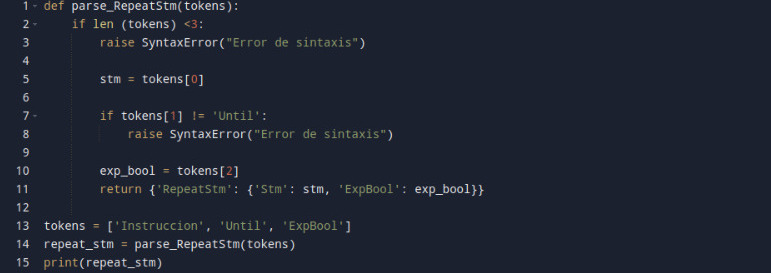
\includegraphics[width=12cm, height=8cm]{images/p1.jpeg}\\
  \item implementación de la semantica de $<PepeatStm>$\\
  De igual manera usaremos python para la implementación de la misma:\\
  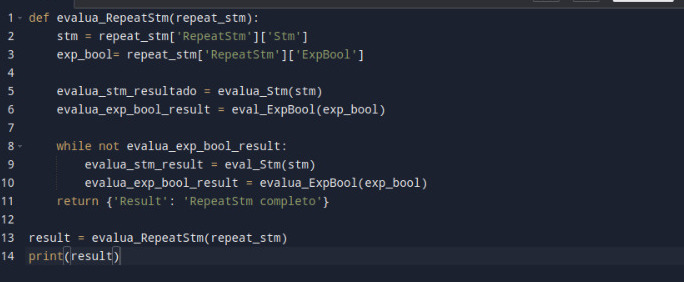
\includegraphics[width=12cm, height=8cm]{images/WhatsApp Image 2023-12-06 at 11.39.25 PM.jpeg}\\
\end{enumerate}



\end{document}